%
% 21-konform.tex -- Konforme Abbildungen
%
% (c) 2026 Prof Dr Andreas Müller
%
\subsection{Konforme Abbildungen}
%
% fig-konform.tex
%
% (c) 2026 Prof Dr Andreas Müller
%
\begin{figure}
\centering
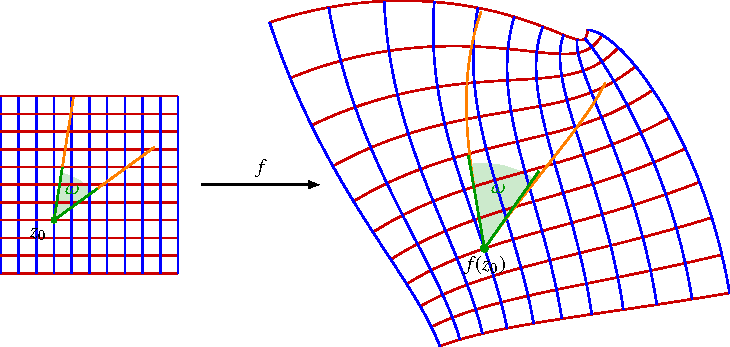
\includegraphics{chapters/020-holomorph/images/konform.pdf}
\caption{Eine holomorph Abbildung $f\colon \mathbb{C}\to\mathbb{C}$
ist konform.
Geraden mit Richtung $w\in\mathbb{C}$, $|w|=1$, durch den Punkt $z_0$
werden auf Kurven ({\color{orange}orange}) durch den Punkt $f(z_0)$
abgebildet, deren Tangenten ({\color{darkgreen}grün}) die Richtung
von $f'(z_0)\cdot w$ haben.
Die Multiplikation mit $f'(z_0)$ ist eine Drehstreckung, die Winkel
erhält.
\label{buch:holomorph:fig:konform}}
\end{figure}
%
Wir betrachten eine holomorphe Abbildung $f\colon U\to\mathbb{C}$ einer
offenen Menge nach $\mathbb{C}$.
Ein Punkt $z_0 \in U$ wird auf $f(z_0)\in\mathbb{C}$ abgebildet.
Die Abbildung~\ref{buch:holomorph:fig:konform} zeigt eine solche Abbildung.
Eine Gerade durch den Punkt $z_0$ kann durch die Richtung $d\in\mathbb{C}$
mit $|d|=1$ geschrieben werden.
Die Gerade besteht aus den Punkten $z_0+dt$ mit $t\in\mathbb{R}$.
Die Bildkurven sind $t\mapsto f(z_0+dt)$.
Die Tangente an die Bildkurve im Punkt $f(z_0)$ hat gemäss der
Ableitung  die Richtung von
\[
f'(z_0) \cdot d.
\]
Da Multiplikation mit $f'(z_0)$ eine Drehstreckung beschreibt, werden
Geraden durch $z_0$, die einen Winkel $\omega$ einschliessen, auf zwei
Tangenten abgebildet, die ebenfalls den Winkel $\omega$ einschliessen.
Folglich bleiben Winkel bei der Abbildung $f$ erhalten, sie ist
\emph{winkeltreu}.
\index{winkeltreu}%

\begin{definition}[konforme Abbildung]
Eine Abbildung, die in jedem Punkt winkeltreue ist,
heisst \emph{konform}.
\index{konform}%
\end{definition}

\begin{satz}
Eine holomorphe Funktion $f\colon U\to\mathbb{C}$ beschreibt in jedem
Punkt $z$, in dem $f'(z)\ne 0$ ist, eine konforme Abbildung.
\end{satz}

Die Gitterlinien stehen im Definitionsgebiet senkrecht aufeinander.
Die rechten Winkel werden von $f$ auf rechte Winkel zwischen den
Bildkurven der Gitterlinien abgebildet.
Daher schneiden sich die Gitterlinien in
Abbildung~\ref{buch:holomorph:fig:konform}
orthogonal.

%
% Nullstellen der Ableitung
%
\subsubsection{Nullstellen der Ableitung}
Bei einer Nullstelle von $f'(z_0)$ sind die Tangentenrichtungen der 
Bildkurven nicht definiert.
Entsprechend ist es nicht sinnvoll davon zu sprechen, dass Winkel bei
der Abbildung erhalten bleiben.
Die Abbildung $z\mapsto f(z) = z^n$ hat in Polarkoordinaten die
Darstellung 
\[
f(re^{i\varphi})
=
r^n e^{in\varphi}
=
r^n(\cos n\varphi + i\sin n\varphi).
\]
Geraden durch den Nullpunkt mit Polarwinkel $\varphi$ werden auf
Geraden durch den Nullpunkt mit Polarwinkel $n\varphi$ abgebildet.
Winkel im Nullpunkt werden also mit $n$ multipliziert.

Wir werden später zeigen, dass eine holomorphe Funktion auch eine 
konvergente Potenzreihe hat.
Hat die Ableitung $f'(z)$ eine Nullstelle im Punkt $z_0$, dann hat
$ g(z) = f(z) - f(z_0) $
eine Potenzreihe, die mit
\[
g(z)
=
\frac{f''(z_0)}{2!}(z-z_0)^2 + o((z-z_0)^2)
\]
beginnt.
Im Punkt $z_0$ werden Winkel daher mit $2$ multipliziert.
Ist die $n$-te Ableitung von $f$ die erste, die im Punkt $z_0$
nicht verschwindet, dann hat $g(z)$ die Potenzreihe
\[
g(z)
=
\frac{f^{(n)}(z_0)}{n!}(z-z_0)^n + o((z-z_0)^n).
\]
Winkel im Punkte $z_0$ werden also mit $n$ multipliziert.

Verwendet man als Definitionsgebiet
$U = \mathbb{C}\setminus\{x\in\mathbb{R} \mid x < 0\}$,
dann kann $z\mapsto f(z)=z^\alpha$ für beliebige rationale $\alpha>0$
durch die Polarformel $f(re^{i\varphi})=r^\alpha e^{i\alpha\varphi}$
definiert werden.
Winkel im Punkt $0$ werden mit $\alpha$ multipliziert.

%
% Winkeltreue Abbildungen sind holomorph
%
\subsubsection{Winkeltreue, orientierungserhaltende Abbildungen sind holomorph}
Eine differenzierbare Abbildung von $U\subset\mathbb{R}^2$ nach $\mathbb{R}^2$
hat die jacobische Matrix $\Jf$ als Ableitung.
Der Winkel zwischen den beiden Vektoren $\vec{u}$ und $\vec{v}$ und
zwischen den Bildvektoren ist
\begin{equation}
\cos
\angle(\vec{u},\vec{v})
=
\frac{\vec{u}\cdot\vec{v}}{|\vec{u}|\cdot |\vec{v}|}
\qquad\text{bzw.}\qquad
\cos
\angle(\Jf \vec{u},\Jf \vec{v})
=
\frac{\Jf \vec{u}\cdot \Jf \vec{v}}{|\Jf\vec{u}|\cdot |\Jf\vec{v}|}.
\label{buch:holomorph:geometrie:coswinkel}
\end{equation}
Sie ist genau dann winkeltreu, wenn die Matrix $\Jf$ das Skalarprodukt
nur mit einem skalaren Faktor $s$ multipliziert, denn dann bleibt der
Kosinus in \eqref{buch:holomorph:geometrie:coswinkel} und damit auch
der Winkel gleich.
Dies ist gleichbedeutend mit der Matrixgleichung
\[
\Jf^t I \Jf
=
\Jf^t \Jf
=
sI
\qquad\Rightarrow\qquad
\biggl(\frac{1}{\!\sqrt{s}}\Jf\biggr)^t
\biggl(\frac{1}{\!\sqrt{s}}\Jf\biggr)
=
I.
\]
Die Matrix
\[
A = \frac{1}{\!\sqrt{s}}\Jf
=
\frac{1}{\!\sqrt{s}}
{\renewcommand{\arraystretch}{2.0}
\begin{pmatrix}
\displaystyle\frac{\partial u}{\partial x} &
\displaystyle\frac{\partial u}{\partial y} \\
\displaystyle\frac{\partial v}{\partial x} &
\displaystyle\frac{\partial v}{\partial y}
\end{pmatrix}}
\]
muss also orthogonal sein.
Ein orthogonale Matrix in zwei Dimensionen ist aber eine Drehtmatrix
oder eine Drehmatrix mit nachfolgender Spiegelung, die die Orientierung
umkehrt.
Falls $\frac{1}{\!\sqrt{s}}\Jf$ eine Drehmatrix ist, folgt
\begin{align}
\frac{1}{\!\sqrt{s}}
{\renewcommand{\arraystretch}{2.0}
\begin{pmatrix}
\displaystyle\frac{\partial u}{\partial x} &
\displaystyle\frac{\partial u}{\partial y} \\
\displaystyle\frac{\partial v}{\partial x} &
\displaystyle\frac{\partial v}{\partial y}
\end{pmatrix}}
&=
\begin{pmatrix}
\cos\varphi&-\sin\varphi\\
\sin\varphi&\phantom{-}\cos\varphi
\end{pmatrix}
\quad\Rightarrow\quad
\left\{
\renewcommand{\arraycolsep}{1.5pt}
\begin{array}{rcccl}
\displaystyle
\frac{\partial u}{\partial x}
&=&
\!\sqrt{s}\cos\varphi
&=&
\displaystyle
\frac{\partial v}{\partial y}
\\[8pt]
\displaystyle
\frac{\partial v}{\partial x}
&=&
\!\sqrt{s}\sin\varphi
&=&
\displaystyle
-\frac{\partial u}{\partial y}
\end{array}
\right.
\label{buch:holomorph:gemetrie:eqn:JfCR}
\end{align}
Die Gleichungen auf der rechten Seite von
\eqref{buch:holomorph:gemetrie:eqn:JfCR}
sind die Cauchy-Riemann-Differential\-glei\-chun\-gen.
\index{Cauchy-Riemann-Differentialgleichungen}%
Damit haben wir den folgenden Satz bewiesen.

\begin{satz}
Ist 
\[
F
\colon
U \to \mathbb{R}^2
:
(x,y) \mapsto \begin{pmatrix} u(x,y)\\v(x,y)\end{pmatrix}
\]
eine differenzierbare Abbildung, die orientierungserhaltend und
winkeltreu ist.
Dann ist die Funktion $f(x+iy) = u(x,y) + iv(x,y)$ eine holomorphe
Funktion.
\end{satz}

